\documentclass[11pt]{article}
\usepackage[textwidth=18.0cm, textheight=23.0cm, top=2.0cm]{geometry}
\usepackage{pst-all}
\usepackage{amssymb}
\usepackage{tikz}
\usepackage{underscore}\begin{document}
\pagestyle{empty}


ClassName: \underline{\textbf{Class_05.2bp-25}}
\par
BinSize: \underline{\textbf{100 × 100}}
\par
ReduceSize: \underline{\textbf{100 × 100}}
\par
TypeNum: \underline{\textbf{60}}
\par
Num: \underline{\textbf{60}}
\par
OutS: \underline{\textbf{160000}}
\par
InS: \underline{\textbf{138657}}
\par
Rate: \underline{\textbf{0.867}}
\par
UB: \underline{\textbf{16}}
\par
LB0: \underline{\textbf{15}}
\par
LB: \underline{\textbf{16}}
\par
LBWithCut: \underline{\textbf{16}}
\par
NodeCut: \underline{\textbf{0}}
\par
ExtendedNodeCnt: \underline{\textbf{1}}
\par
GenNodeCnt: \underline{\textbf{1}}
\par
PrimalNode: \underline{\textbf{0}}
\par
ColumnCount: \underline{\textbf{167}}
\par
TotalCutCount: \underline{\textbf{0}}
\par
RootCutCount: \underline{\textbf{0}}
\par
LPSolverCnt: \underline{\textbf{152}}
\par
PricingSolverCnt: \underline{\textbf{152}}
\par
BranchAndBoundNum: \underline{\textbf{1}}
\par
isOpt: \underline{\textbf{true}}
\par
TimeOnInitSolution: \underline{\textbf{600.000 s}}
\par
TimeOnPrimal: \underline{\textbf{0.000 s}}
\par
TimeOnPricing: \underline{\textbf{379.816 s}}
\par
TimeOnRmp: \underline{\textbf{0.172 s}}
\par
TotalTime: \underline{\textbf{980.350 s}}
\par
\newpage


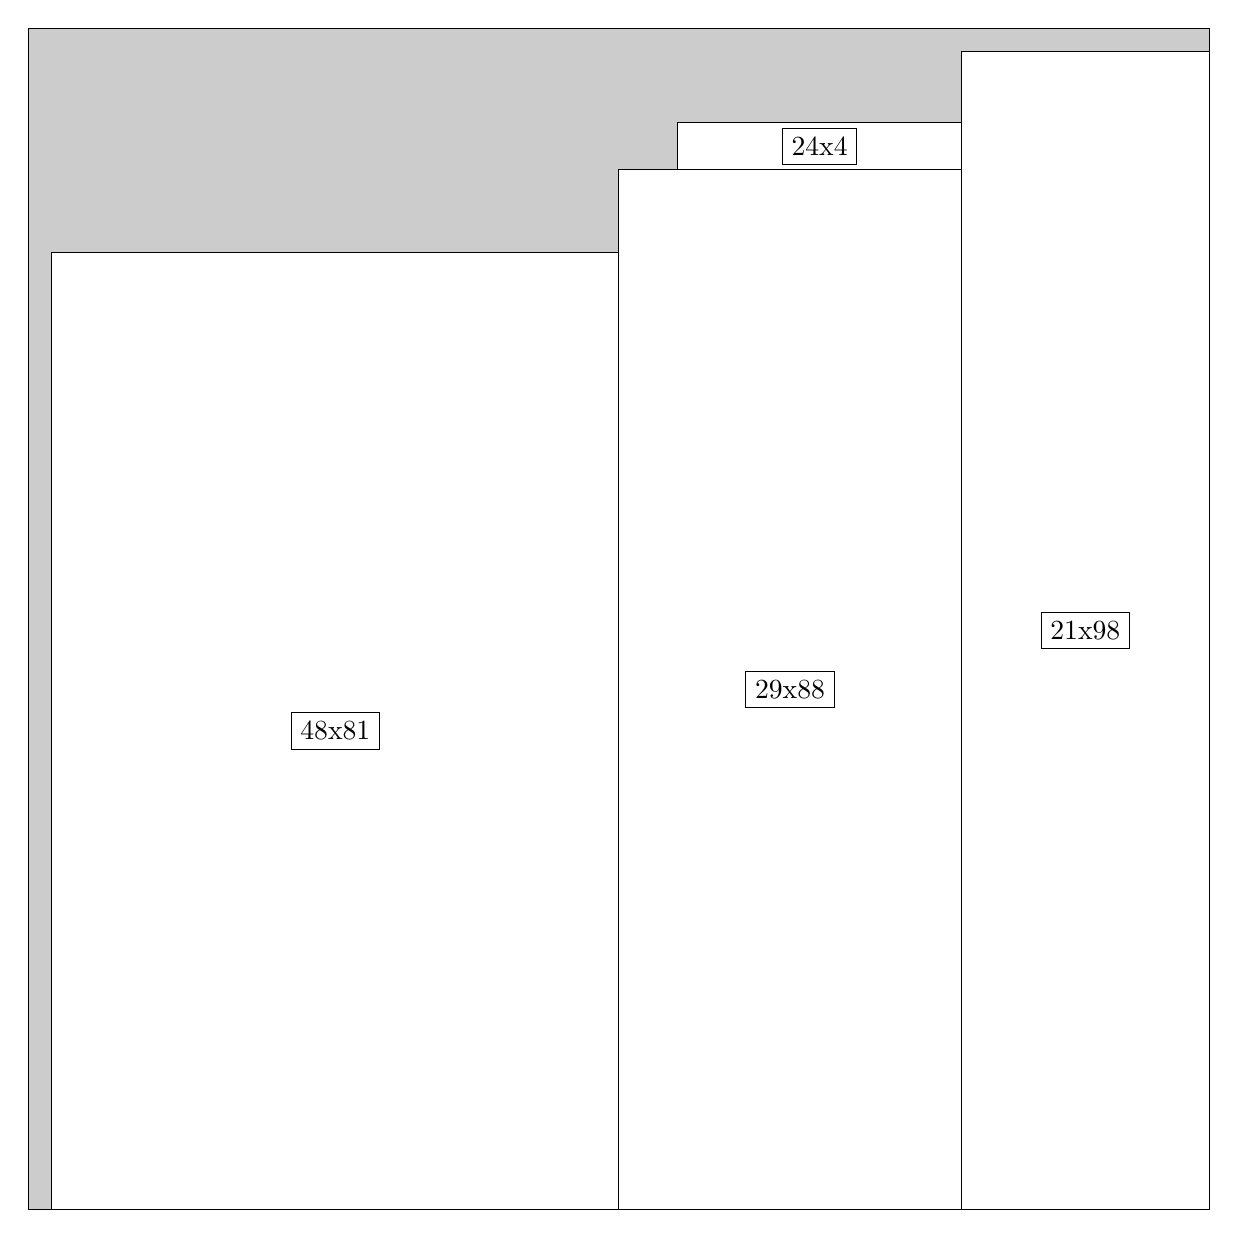
\begin{tikzpicture}[shorten >=1pt,scale=1.0,every node/.style={scale=1.0},->]
\tikzstyle{vertex}=[circle,fill=black!25,minimum size=14pt,inner sep=0pt]
\filldraw[fill=gray!40!white, draw=black] (0,0) rectangle (15.0,15.0);
\foreach \name/\x/\y/\w/\h in {21x98/11.85/0.0/3.15/14.7,29x88/7.5/0.0/4.35/13.2,24x4/8.25/13.2/3.5999999999999996/0.6,48x81/0.3/0.0/7.199999999999999/12.15}
\filldraw[fill=white!40!white, draw=black] (\x,\y) rectangle node[draw] (\name) {\name} ++(\w,\h);
\end{tikzpicture}


w =21 , h =98 , x =79 , y =0 , v =2058
\par
w =29 , h =88 , x =50 , y =0 , v =2552
\par
w =24 , h =4 , x =55 , y =88 , v =96
\par
w =48 , h =81 , x =2 , y =0 , v =3888
\par
\newpage


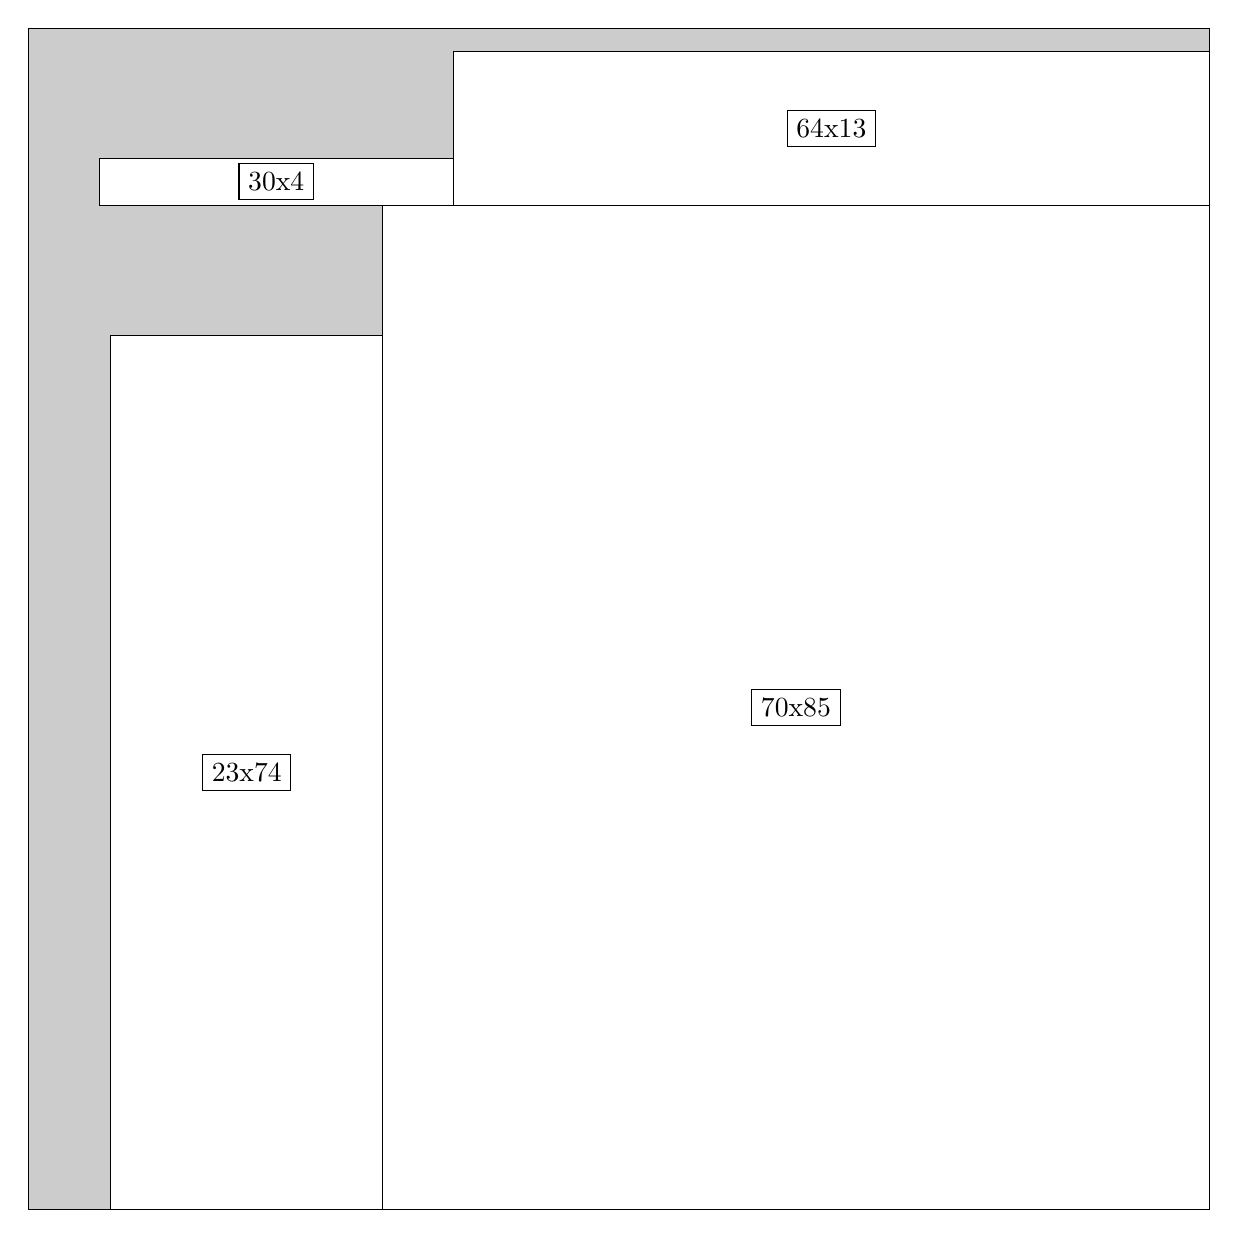
\begin{tikzpicture}[shorten >=1pt,scale=1.0,every node/.style={scale=1.0},->]
\tikzstyle{vertex}=[circle,fill=black!25,minimum size=14pt,inner sep=0pt]
\filldraw[fill=gray!40!white, draw=black] (0,0) rectangle (15.0,15.0);
\foreach \name/\x/\y/\w/\h in {70x85/4.5/0.0/10.5/12.75,23x74/1.05/0.0/3.4499999999999997/11.1,64x13/5.3999999999999995/12.75/9.6/1.95,30x4/0.8999999999999999/12.75/4.5/0.6}
\filldraw[fill=white!40!white, draw=black] (\x,\y) rectangle node[draw] (\name) {\name} ++(\w,\h);
\end{tikzpicture}


w =70 , h =85 , x =30 , y =0 , v =5950
\par
w =23 , h =74 , x =7 , y =0 , v =1702
\par
w =64 , h =13 , x =36 , y =85 , v =832
\par
w =30 , h =4 , x =6 , y =85 , v =120
\par
\newpage


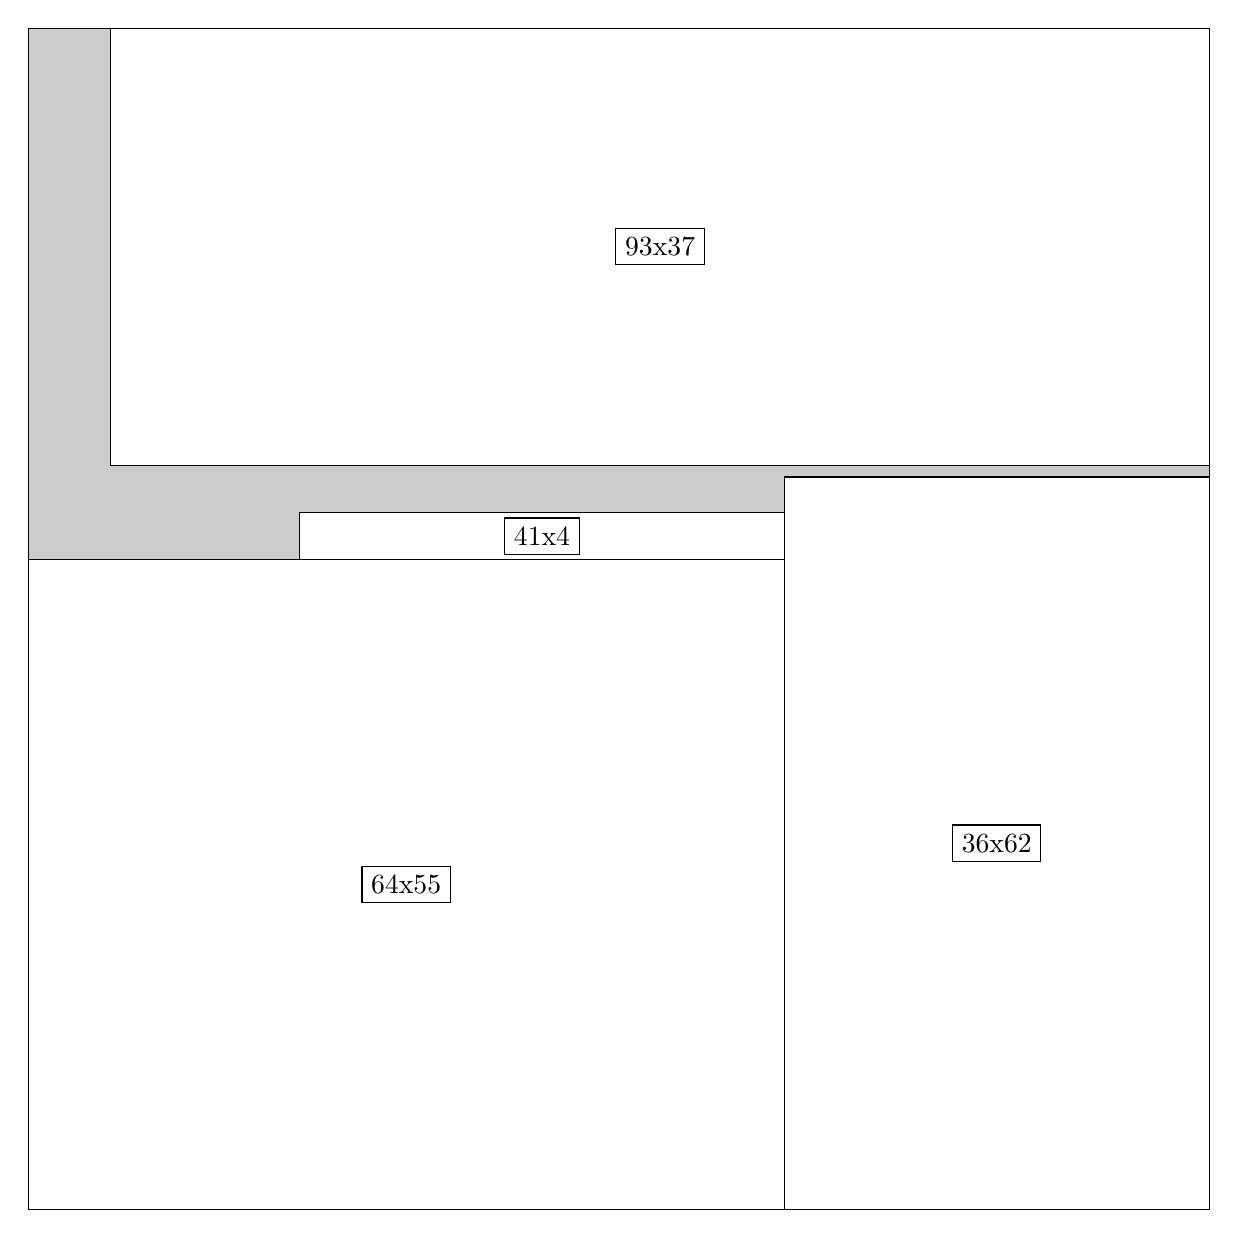
\begin{tikzpicture}[shorten >=1pt,scale=1.0,every node/.style={scale=1.0},->]
\tikzstyle{vertex}=[circle,fill=black!25,minimum size=14pt,inner sep=0pt]
\filldraw[fill=gray!40!white, draw=black] (0,0) rectangle (15.0,15.0);
\foreach \name/\x/\y/\w/\h in {36x62/9.6/0.0/5.3999999999999995/9.299999999999999,64x55/0.0/0.0/9.6/8.25,41x4/3.4499999999999997/8.25/6.1499999999999995/0.6,93x37/1.05/9.45/13.95/5.55}
\filldraw[fill=white!40!white, draw=black] (\x,\y) rectangle node[draw] (\name) {\name} ++(\w,\h);
\end{tikzpicture}


w =36 , h =62 , x =64 , y =0 , v =2232
\par
w =64 , h =55 , x =0 , y =0 , v =3520
\par
w =41 , h =4 , x =23 , y =55 , v =164
\par
w =93 , h =37 , x =7 , y =63 , v =3441
\par
\newpage


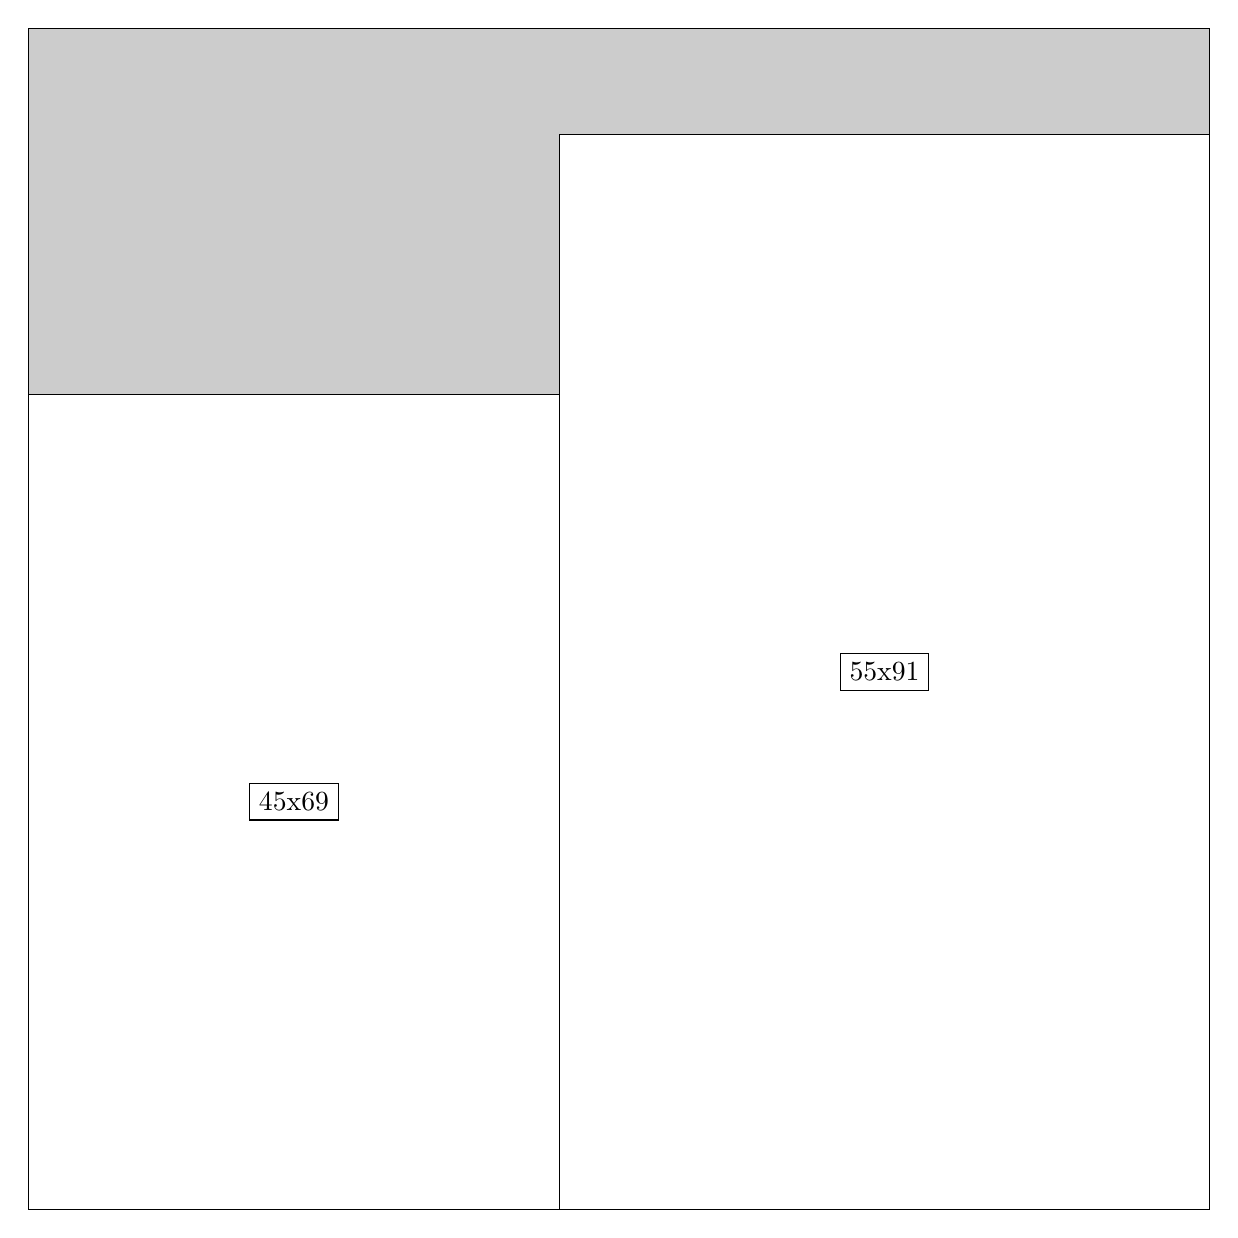
\begin{tikzpicture}[shorten >=1pt,scale=1.0,every node/.style={scale=1.0},->]
\tikzstyle{vertex}=[circle,fill=black!25,minimum size=14pt,inner sep=0pt]
\filldraw[fill=gray!40!white, draw=black] (0,0) rectangle (15.0,15.0);
\foreach \name/\x/\y/\w/\h in {55x91/6.75/0.0/8.25/13.65,45x69/0.0/0.0/6.75/10.35}
\filldraw[fill=white!40!white, draw=black] (\x,\y) rectangle node[draw] (\name) {\name} ++(\w,\h);
\end{tikzpicture}


w =55 , h =91 , x =45 , y =0 , v =5005
\par
w =45 , h =69 , x =0 , y =0 , v =3105
\par
\newpage


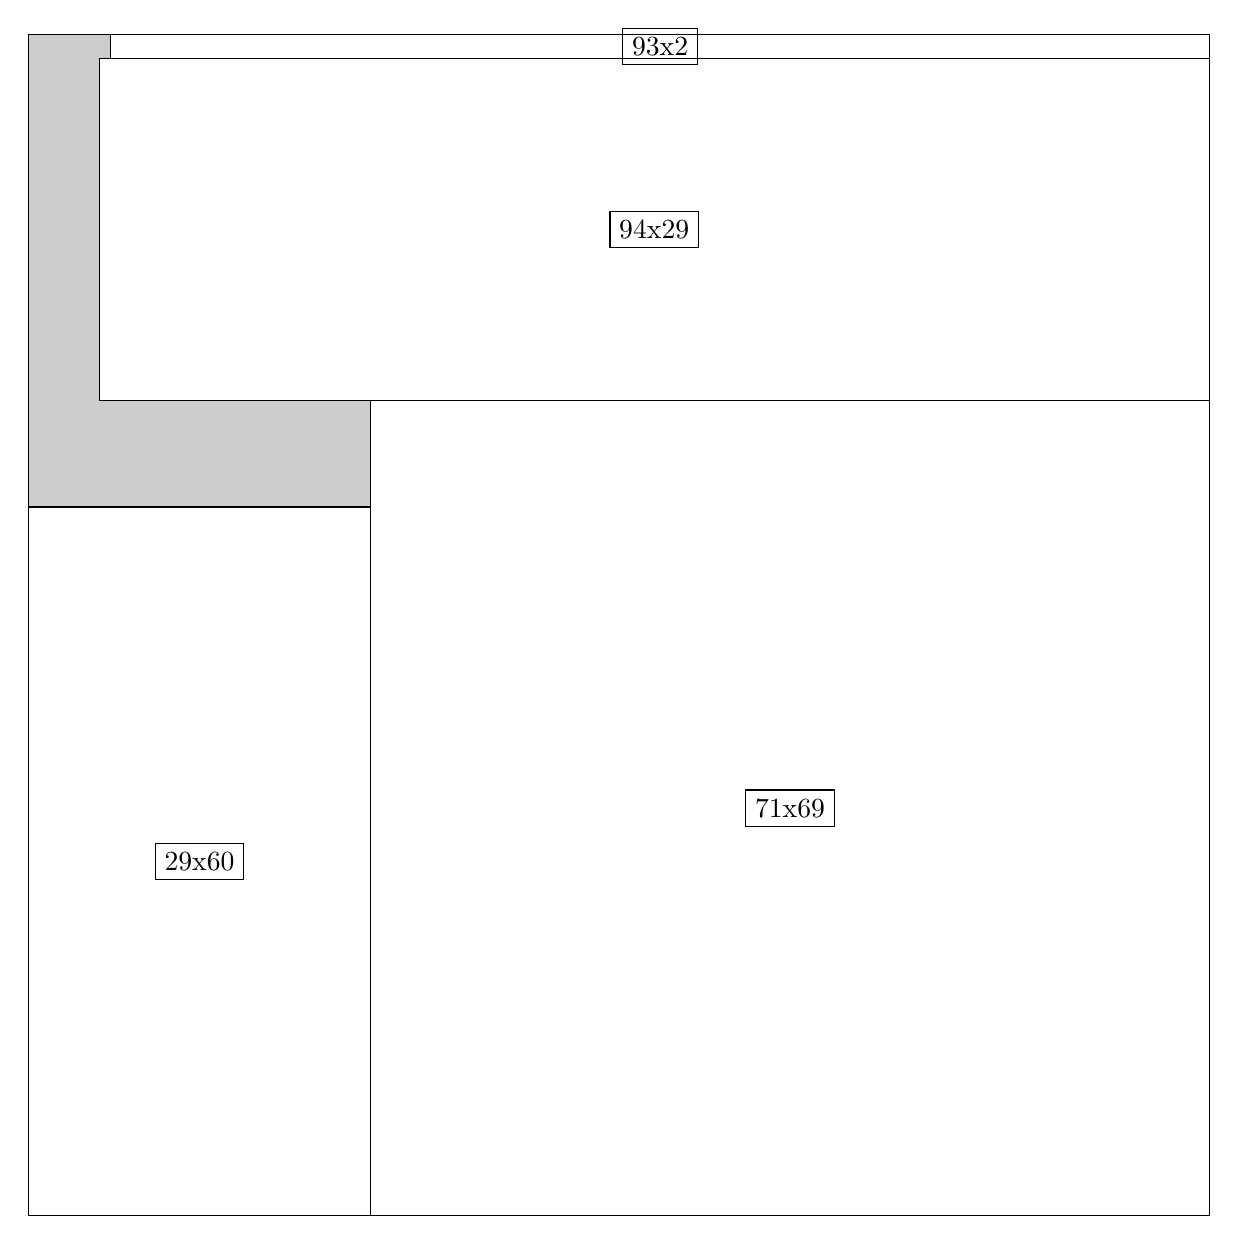
\begin{tikzpicture}[shorten >=1pt,scale=1.0,every node/.style={scale=1.0},->]
\tikzstyle{vertex}=[circle,fill=black!25,minimum size=14pt,inner sep=0pt]
\filldraw[fill=gray!40!white, draw=black] (0,0) rectangle (15.0,15.0);
\foreach \name/\x/\y/\w/\h in {71x69/4.35/0.0/10.65/10.35,29x60/0.0/0.0/4.35/9.0,94x29/0.8999999999999999/10.35/14.1/4.35,93x2/1.05/14.7/13.95/0.3}
\filldraw[fill=white!40!white, draw=black] (\x,\y) rectangle node[draw] (\name) {\name} ++(\w,\h);
\end{tikzpicture}


w =71 , h =69 , x =29 , y =0 , v =4899
\par
w =29 , h =60 , x =0 , y =0 , v =1740
\par
w =94 , h =29 , x =6 , y =69 , v =2726
\par
w =93 , h =2 , x =7 , y =98 , v =186
\par
\newpage


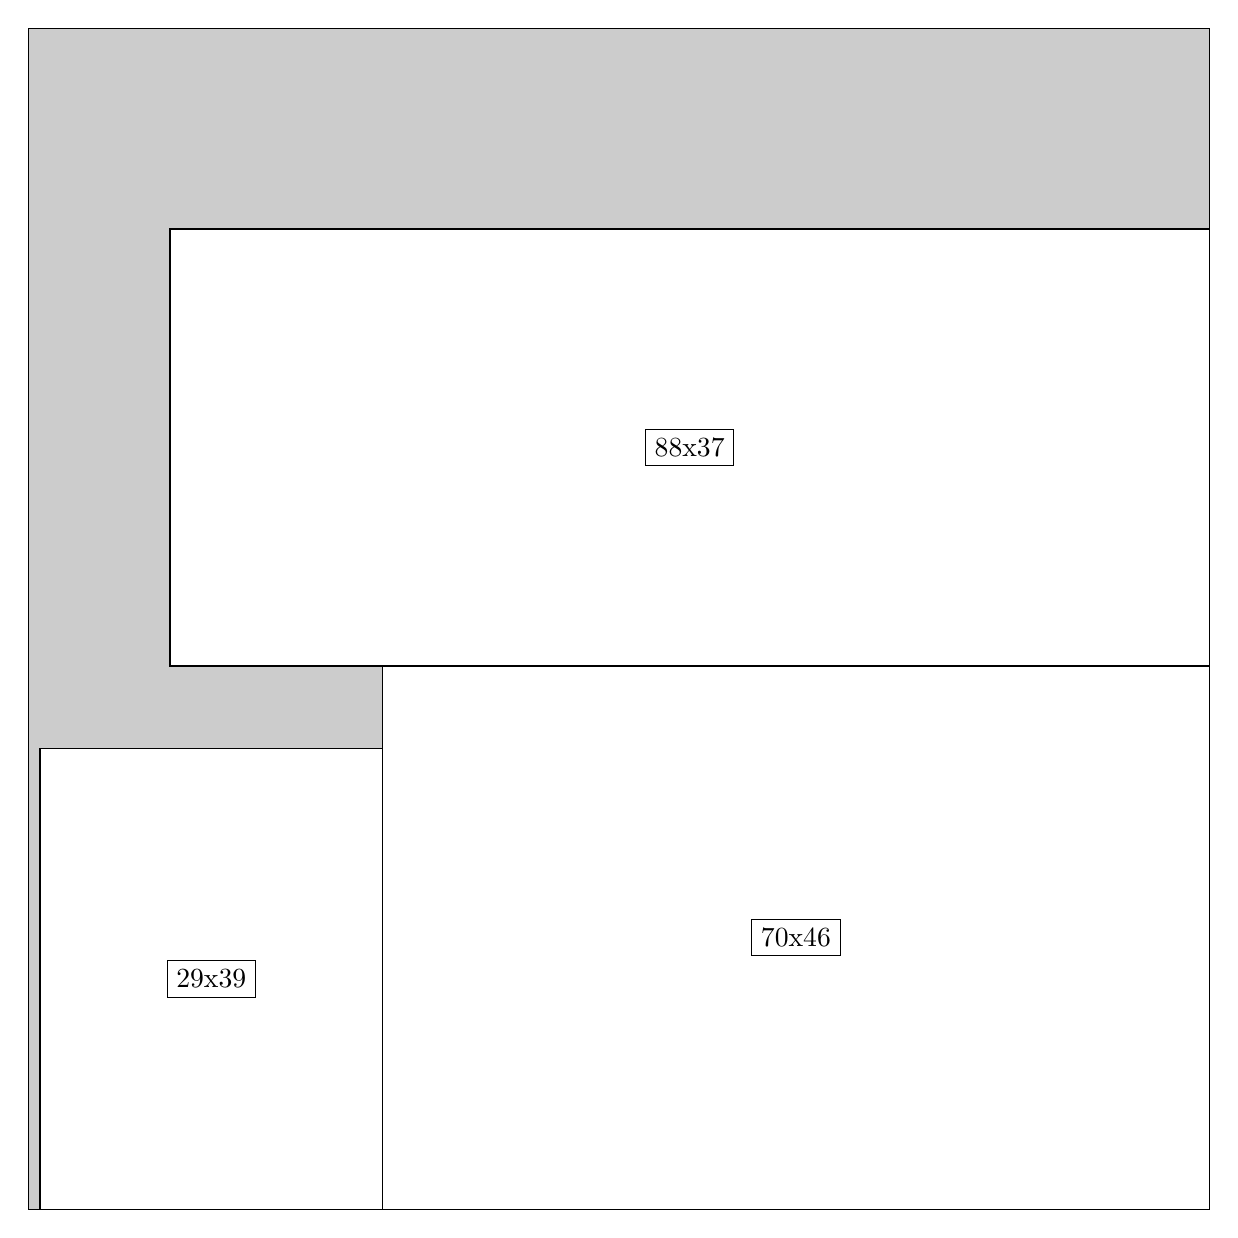
\begin{tikzpicture}[shorten >=1pt,scale=1.0,every node/.style={scale=1.0},->]
\tikzstyle{vertex}=[circle,fill=black!25,minimum size=14pt,inner sep=0pt]
\filldraw[fill=gray!40!white, draw=black] (0,0) rectangle (15.0,15.0);
\foreach \name/\x/\y/\w/\h in {70x46/4.5/0.0/10.5/6.8999999999999995,29x39/0.15/0.0/4.35/5.85,88x37/1.7999999999999998/6.8999999999999995/13.2/5.55}
\filldraw[fill=white!40!white, draw=black] (\x,\y) rectangle node[draw] (\name) {\name} ++(\w,\h);
\end{tikzpicture}


w =70 , h =46 , x =30 , y =0 , v =3220
\par
w =29 , h =39 , x =1 , y =0 , v =1131
\par
w =88 , h =37 , x =12 , y =46 , v =3256
\par
\newpage


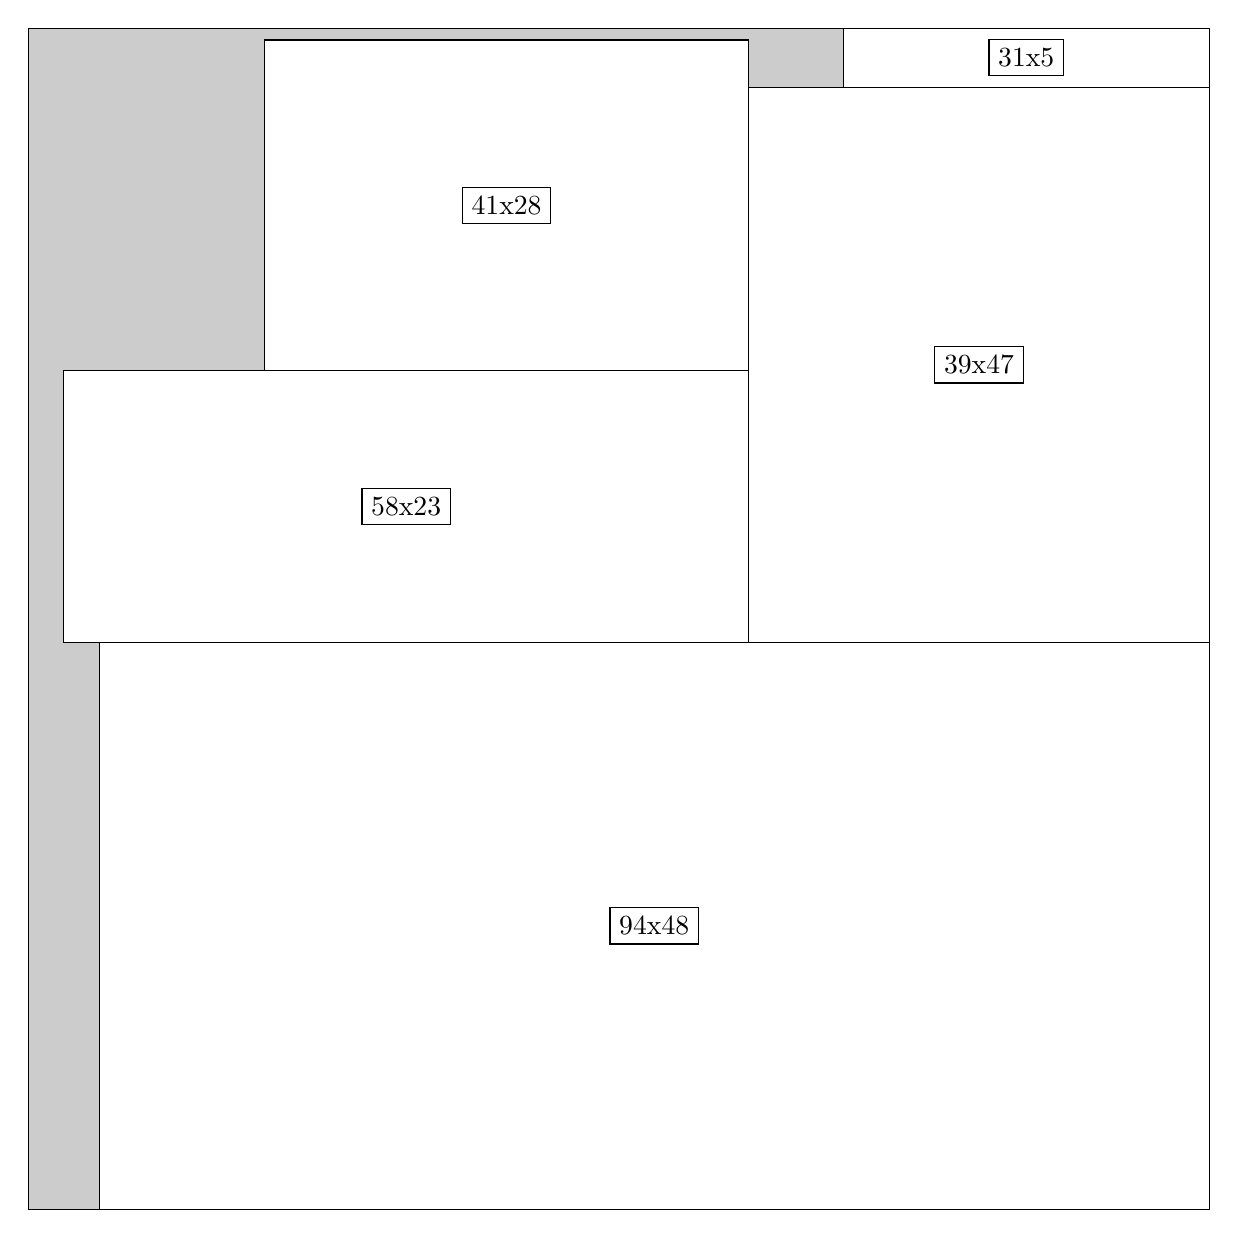
\begin{tikzpicture}[shorten >=1pt,scale=1.0,every node/.style={scale=1.0},->]
\tikzstyle{vertex}=[circle,fill=black!25,minimum size=14pt,inner sep=0pt]
\filldraw[fill=gray!40!white, draw=black] (0,0) rectangle (15.0,15.0);
\foreach \name/\x/\y/\w/\h in {94x48/0.8999999999999999/0.0/14.1/7.199999999999999,39x47/9.15/7.199999999999999/5.85/7.05,31x5/10.35/14.25/4.6499999999999995/0.75,58x23/0.44999999999999996/7.199999999999999/8.7/3.4499999999999997,41x28/3.0/10.65/6.1499999999999995/4.2}
\filldraw[fill=white!40!white, draw=black] (\x,\y) rectangle node[draw] (\name) {\name} ++(\w,\h);
\end{tikzpicture}


w =94 , h =48 , x =6 , y =0 , v =4512
\par
w =39 , h =47 , x =61 , y =48 , v =1833
\par
w =31 , h =5 , x =69 , y =95 , v =155
\par
w =58 , h =23 , x =3 , y =48 , v =1334
\par
w =41 , h =28 , x =20 , y =71 , v =1148
\par
\newpage


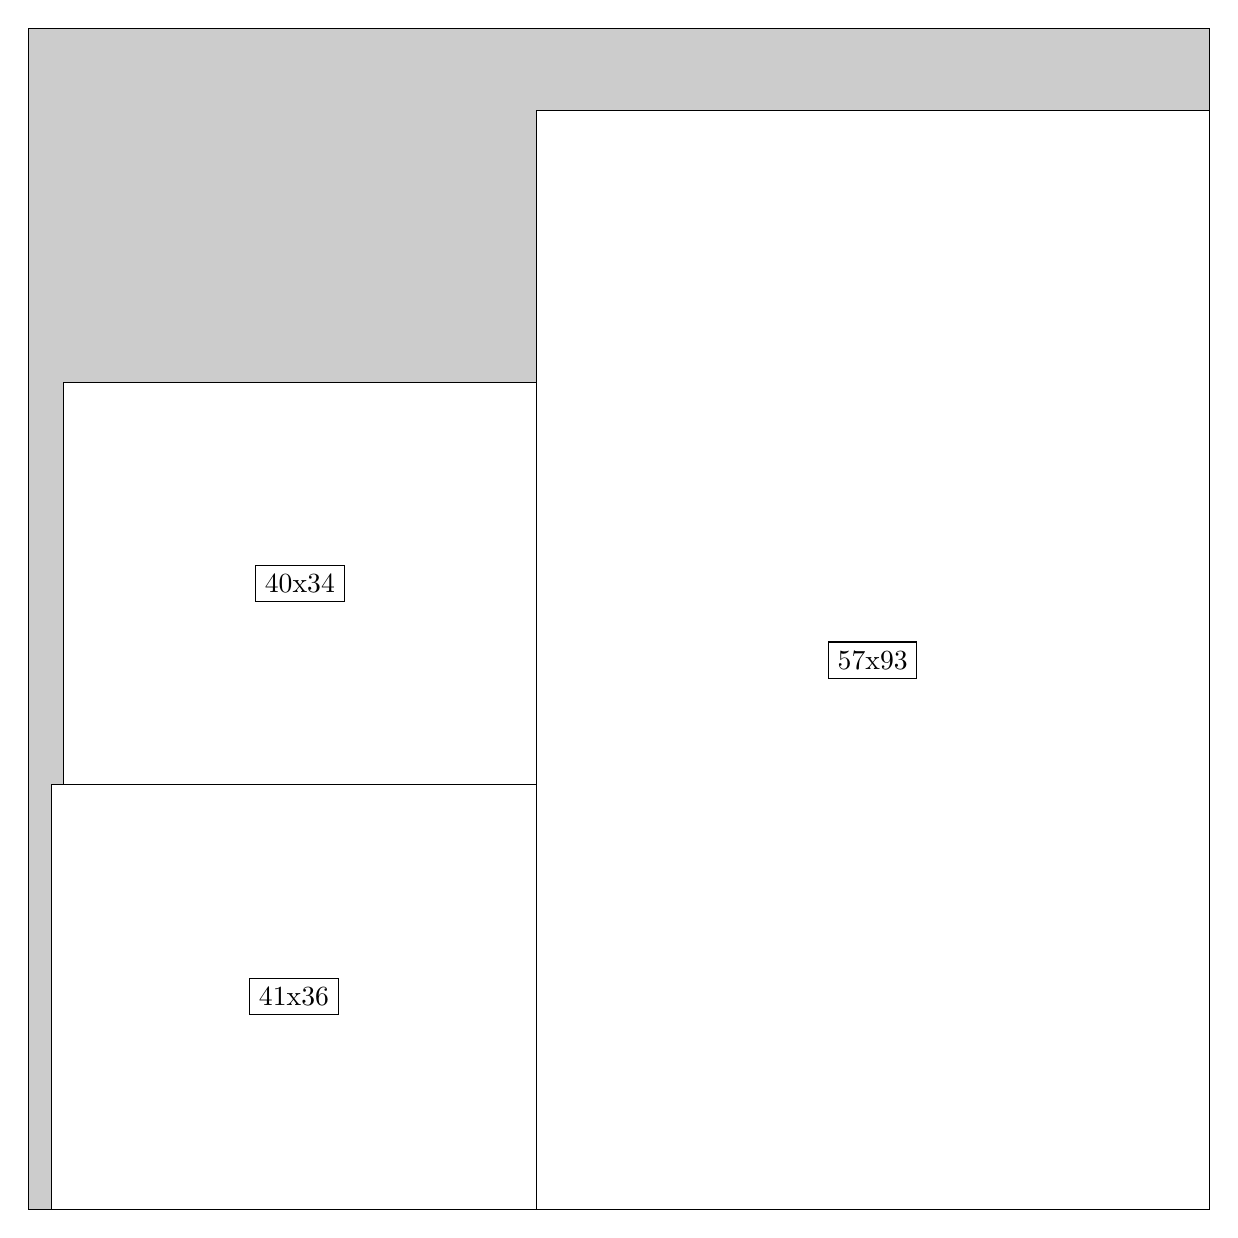
\begin{tikzpicture}[shorten >=1pt,scale=1.0,every node/.style={scale=1.0},->]
\tikzstyle{vertex}=[circle,fill=black!25,minimum size=14pt,inner sep=0pt]
\filldraw[fill=gray!40!white, draw=black] (0,0) rectangle (15.0,15.0);
\foreach \name/\x/\y/\w/\h in {57x93/6.45/0.0/8.549999999999999/13.95,41x36/0.3/0.0/6.1499999999999995/5.3999999999999995,40x34/0.44999999999999996/5.3999999999999995/6.0/5.1}
\filldraw[fill=white!40!white, draw=black] (\x,\y) rectangle node[draw] (\name) {\name} ++(\w,\h);
\end{tikzpicture}


w =57 , h =93 , x =43 , y =0 , v =5301
\par
w =41 , h =36 , x =2 , y =0 , v =1476
\par
w =40 , h =34 , x =3 , y =36 , v =1360
\par
\newpage


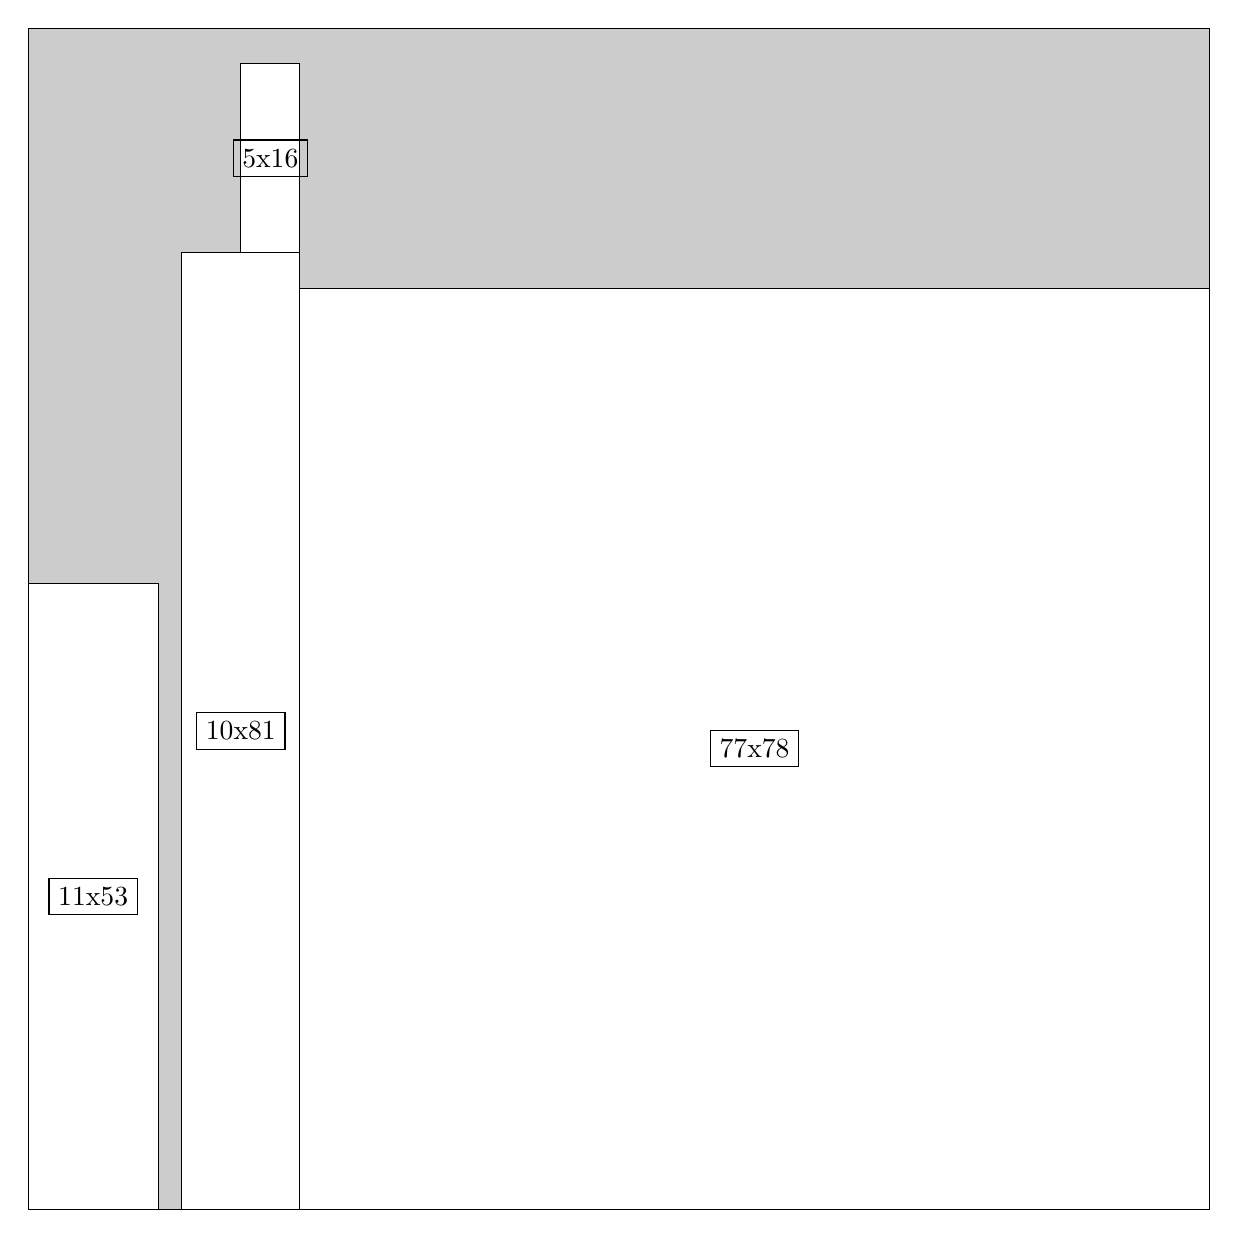
\begin{tikzpicture}[shorten >=1pt,scale=1.0,every node/.style={scale=1.0},->]
\tikzstyle{vertex}=[circle,fill=black!25,minimum size=14pt,inner sep=0pt]
\filldraw[fill=gray!40!white, draw=black] (0,0) rectangle (15.0,15.0);
\foreach \name/\x/\y/\w/\h in {77x78/3.4499999999999997/0.0/11.549999999999999/11.7,10x81/1.95/0.0/1.5/12.15,5x16/2.6999999999999997/12.15/0.75/2.4,11x53/0.0/0.0/1.65/7.949999999999999}
\filldraw[fill=white!40!white, draw=black] (\x,\y) rectangle node[draw] (\name) {\name} ++(\w,\h);
\end{tikzpicture}


w =77 , h =78 , x =23 , y =0 , v =6006
\par
w =10 , h =81 , x =13 , y =0 , v =810
\par
w =5 , h =16 , x =18 , y =81 , v =80
\par
w =11 , h =53 , x =0 , y =0 , v =583
\par
\newpage


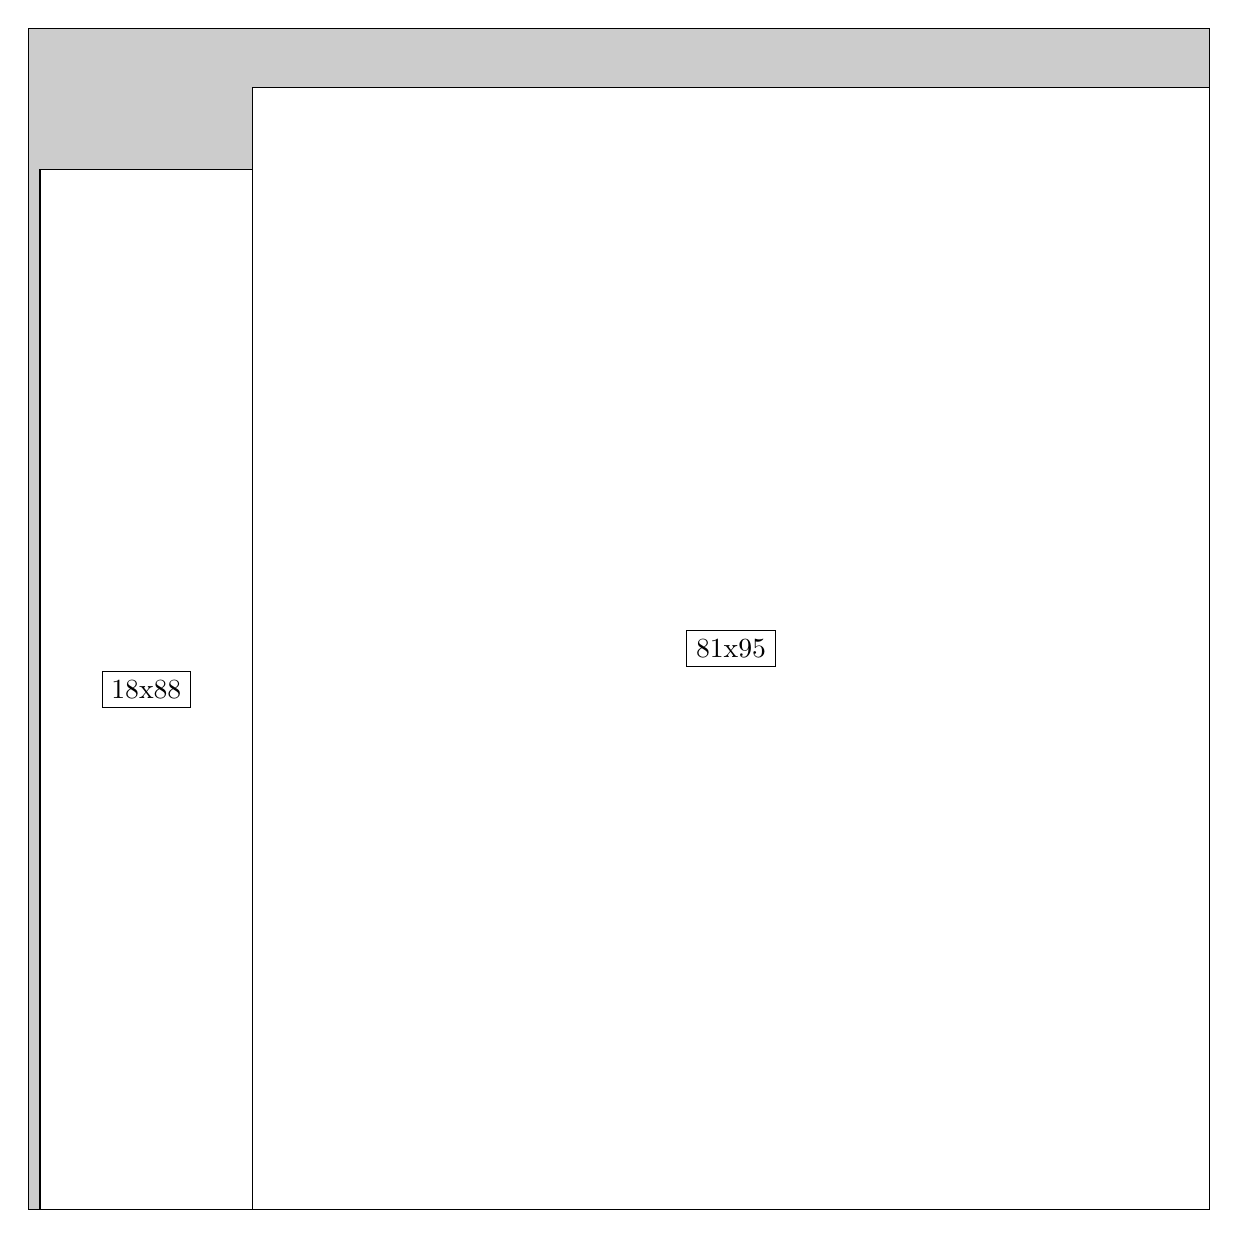
\begin{tikzpicture}[shorten >=1pt,scale=1.0,every node/.style={scale=1.0},->]
\tikzstyle{vertex}=[circle,fill=black!25,minimum size=14pt,inner sep=0pt]
\filldraw[fill=gray!40!white, draw=black] (0,0) rectangle (15.0,15.0);
\foreach \name/\x/\y/\w/\h in {81x95/2.85/0.0/12.15/14.25,18x88/0.15/0.0/2.6999999999999997/13.2}
\filldraw[fill=white!40!white, draw=black] (\x,\y) rectangle node[draw] (\name) {\name} ++(\w,\h);
\end{tikzpicture}


w =81 , h =95 , x =19 , y =0 , v =7695
\par
w =18 , h =88 , x =1 , y =0 , v =1584
\par
\newpage


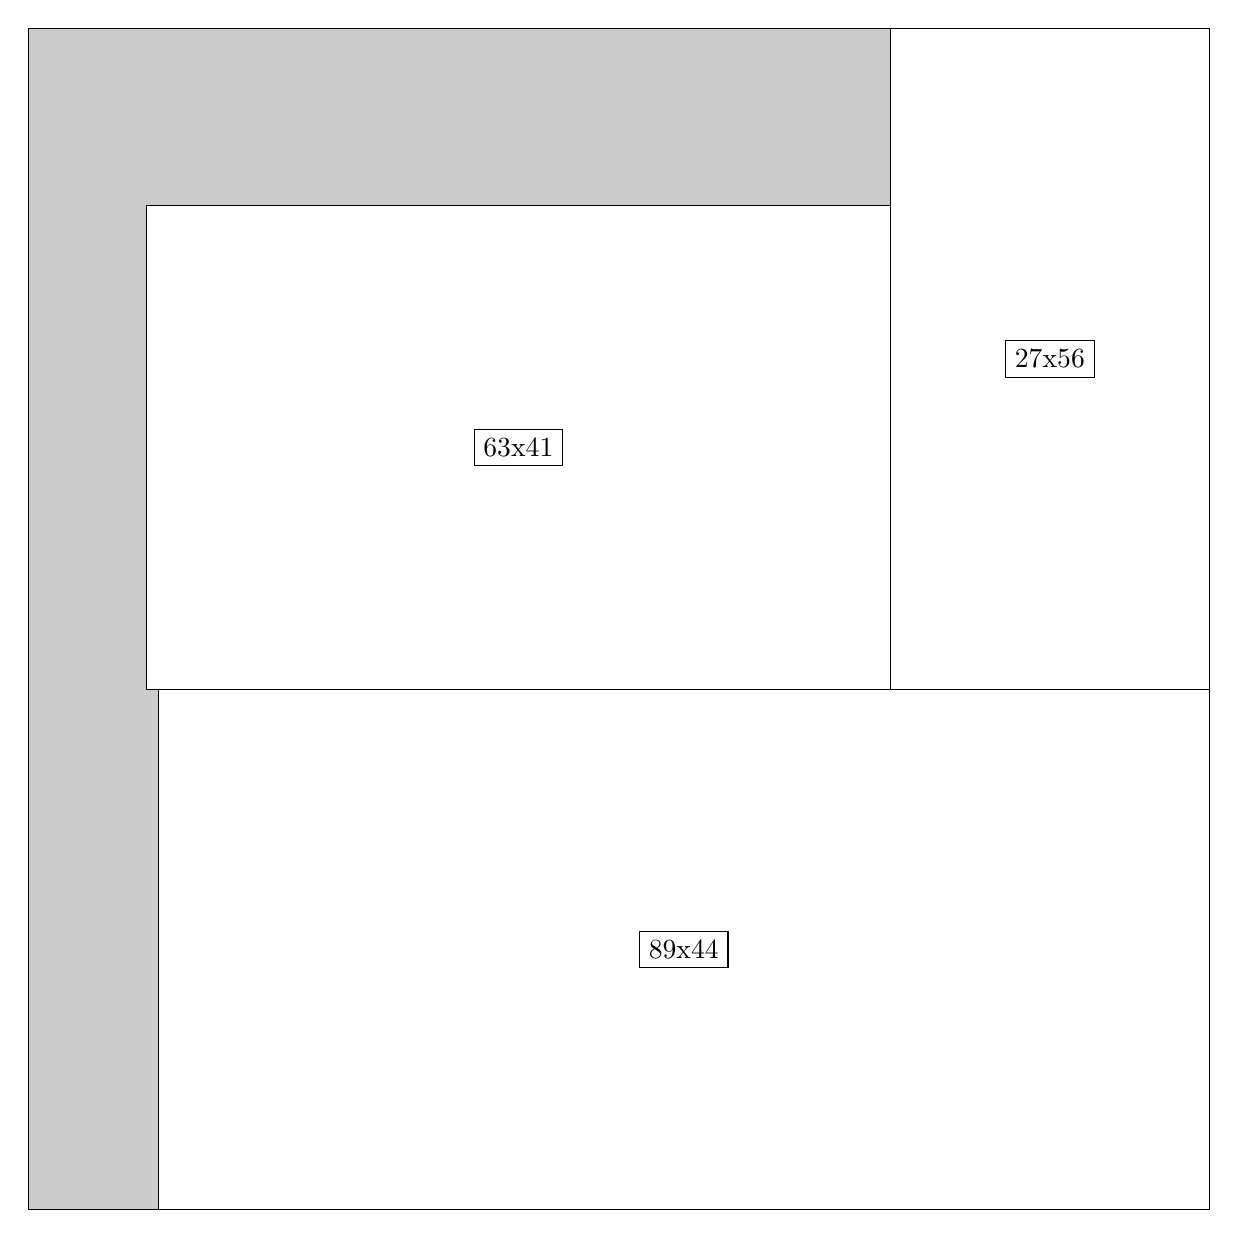
\begin{tikzpicture}[shorten >=1pt,scale=1.0,every node/.style={scale=1.0},->]
\tikzstyle{vertex}=[circle,fill=black!25,minimum size=14pt,inner sep=0pt]
\filldraw[fill=gray!40!white, draw=black] (0,0) rectangle (15.0,15.0);
\foreach \name/\x/\y/\w/\h in {89x44/1.65/0.0/13.35/6.6,27x56/10.95/6.6/4.05/8.4,63x41/1.5/6.6/9.45/6.1499999999999995}
\filldraw[fill=white!40!white, draw=black] (\x,\y) rectangle node[draw] (\name) {\name} ++(\w,\h);
\end{tikzpicture}


w =89 , h =44 , x =11 , y =0 , v =3916
\par
w =27 , h =56 , x =73 , y =44 , v =1512
\par
w =63 , h =41 , x =10 , y =44 , v =2583
\par
\newpage


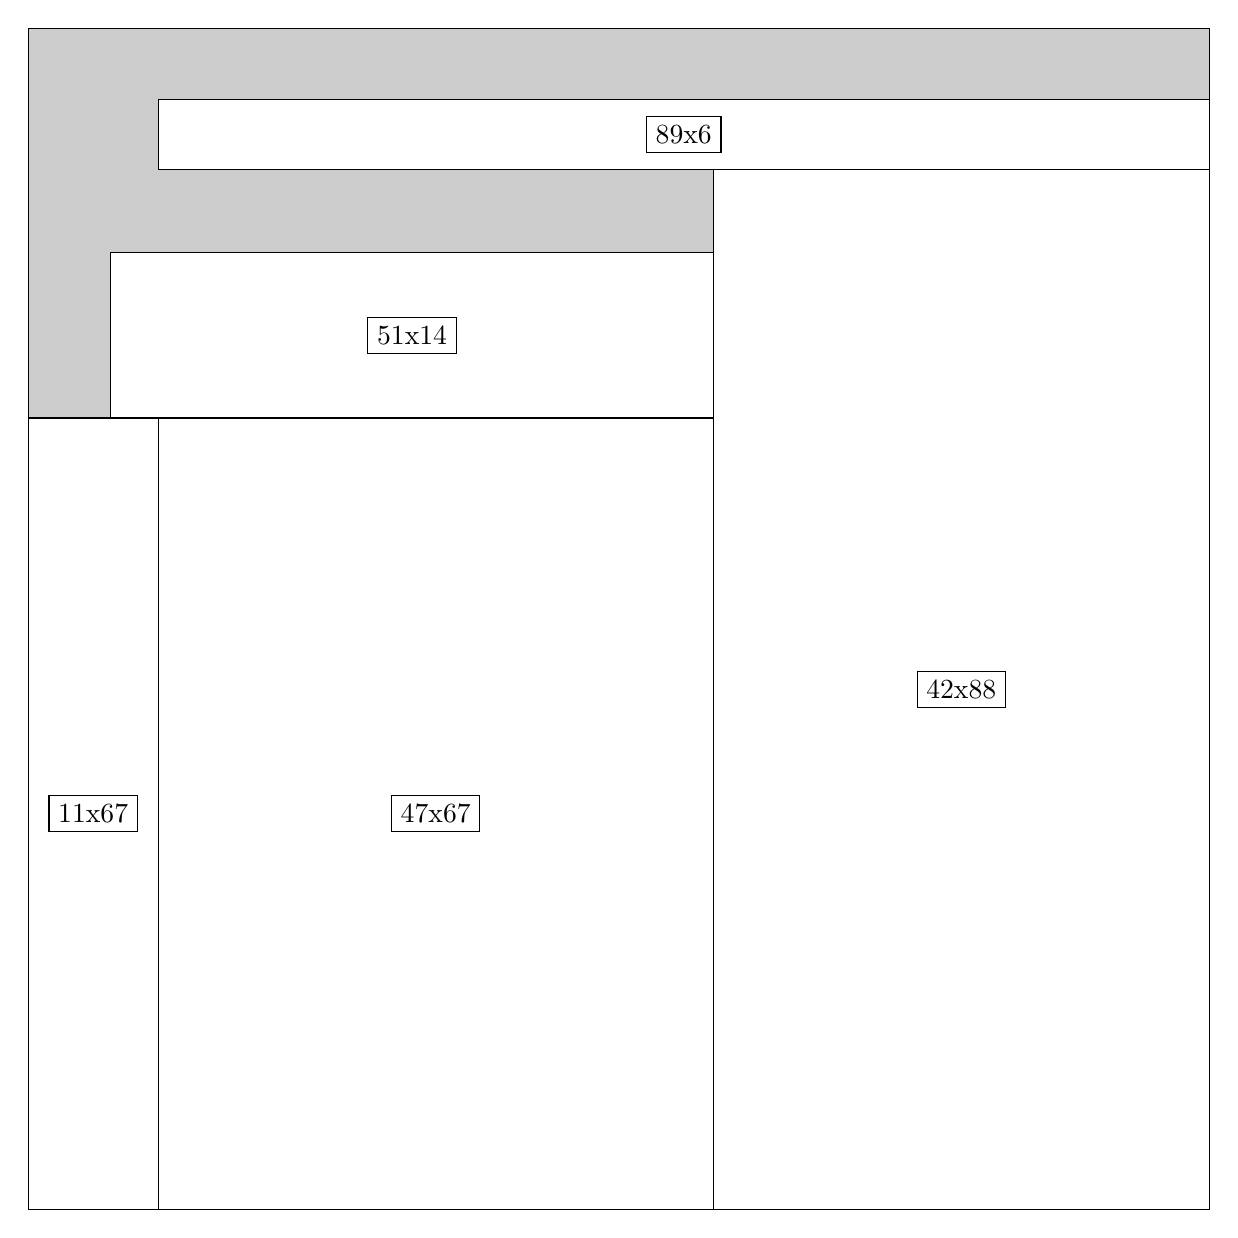
\begin{tikzpicture}[shorten >=1pt,scale=1.0,every node/.style={scale=1.0},->]
\tikzstyle{vertex}=[circle,fill=black!25,minimum size=14pt,inner sep=0pt]
\filldraw[fill=gray!40!white, draw=black] (0,0) rectangle (15.0,15.0);
\foreach \name/\x/\y/\w/\h in {42x88/8.7/0.0/6.3/13.2,47x67/1.65/0.0/7.05/10.049999999999999,11x67/0.0/0.0/1.65/10.049999999999999,51x14/1.05/10.049999999999999/7.6499999999999995/2.1,89x6/1.65/13.2/13.35/0.8999999999999999}
\filldraw[fill=white!40!white, draw=black] (\x,\y) rectangle node[draw] (\name) {\name} ++(\w,\h);
\end{tikzpicture}


w =42 , h =88 , x =58 , y =0 , v =3696
\par
w =47 , h =67 , x =11 , y =0 , v =3149
\par
w =11 , h =67 , x =0 , y =0 , v =737
\par
w =51 , h =14 , x =7 , y =67 , v =714
\par
w =89 , h =6 , x =11 , y =88 , v =534
\par
\newpage


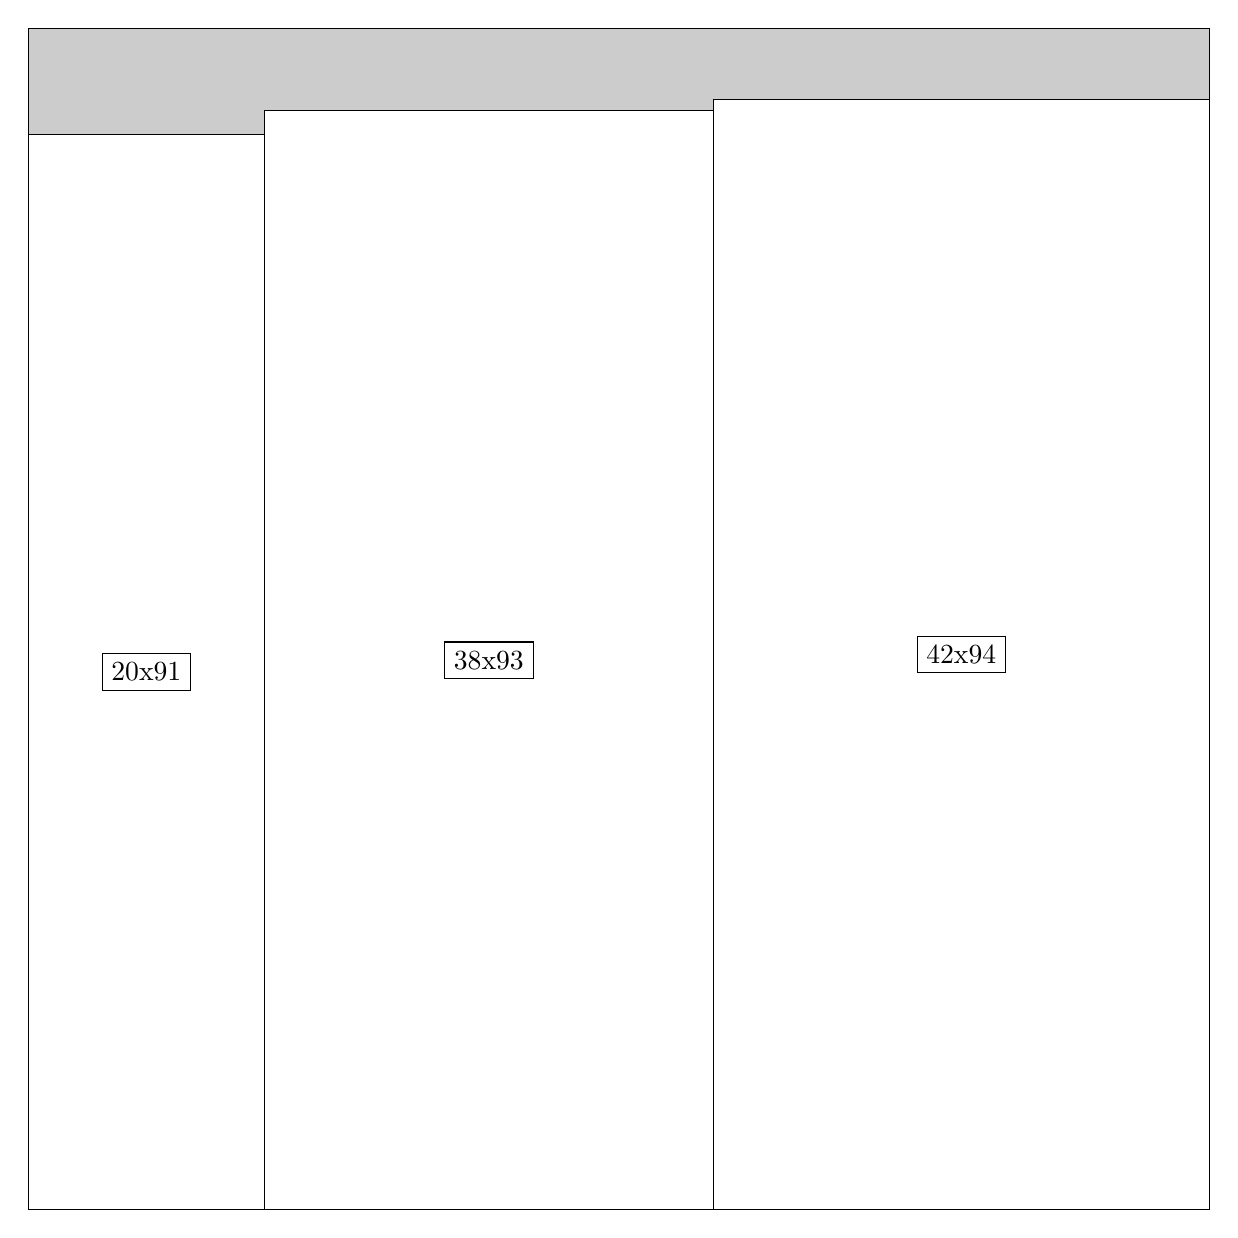
\begin{tikzpicture}[shorten >=1pt,scale=1.0,every node/.style={scale=1.0},->]
\tikzstyle{vertex}=[circle,fill=black!25,minimum size=14pt,inner sep=0pt]
\filldraw[fill=gray!40!white, draw=black] (0,0) rectangle (15.0,15.0);
\foreach \name/\x/\y/\w/\h in {42x94/8.7/0.0/6.3/14.1,38x93/3.0/0.0/5.7/13.95,20x91/0.0/0.0/3.0/13.65}
\filldraw[fill=white!40!white, draw=black] (\x,\y) rectangle node[draw] (\name) {\name} ++(\w,\h);
\end{tikzpicture}


w =42 , h =94 , x =58 , y =0 , v =3948
\par
w =38 , h =93 , x =20 , y =0 , v =3534
\par
w =20 , h =91 , x =0 , y =0 , v =1820
\par
\newpage


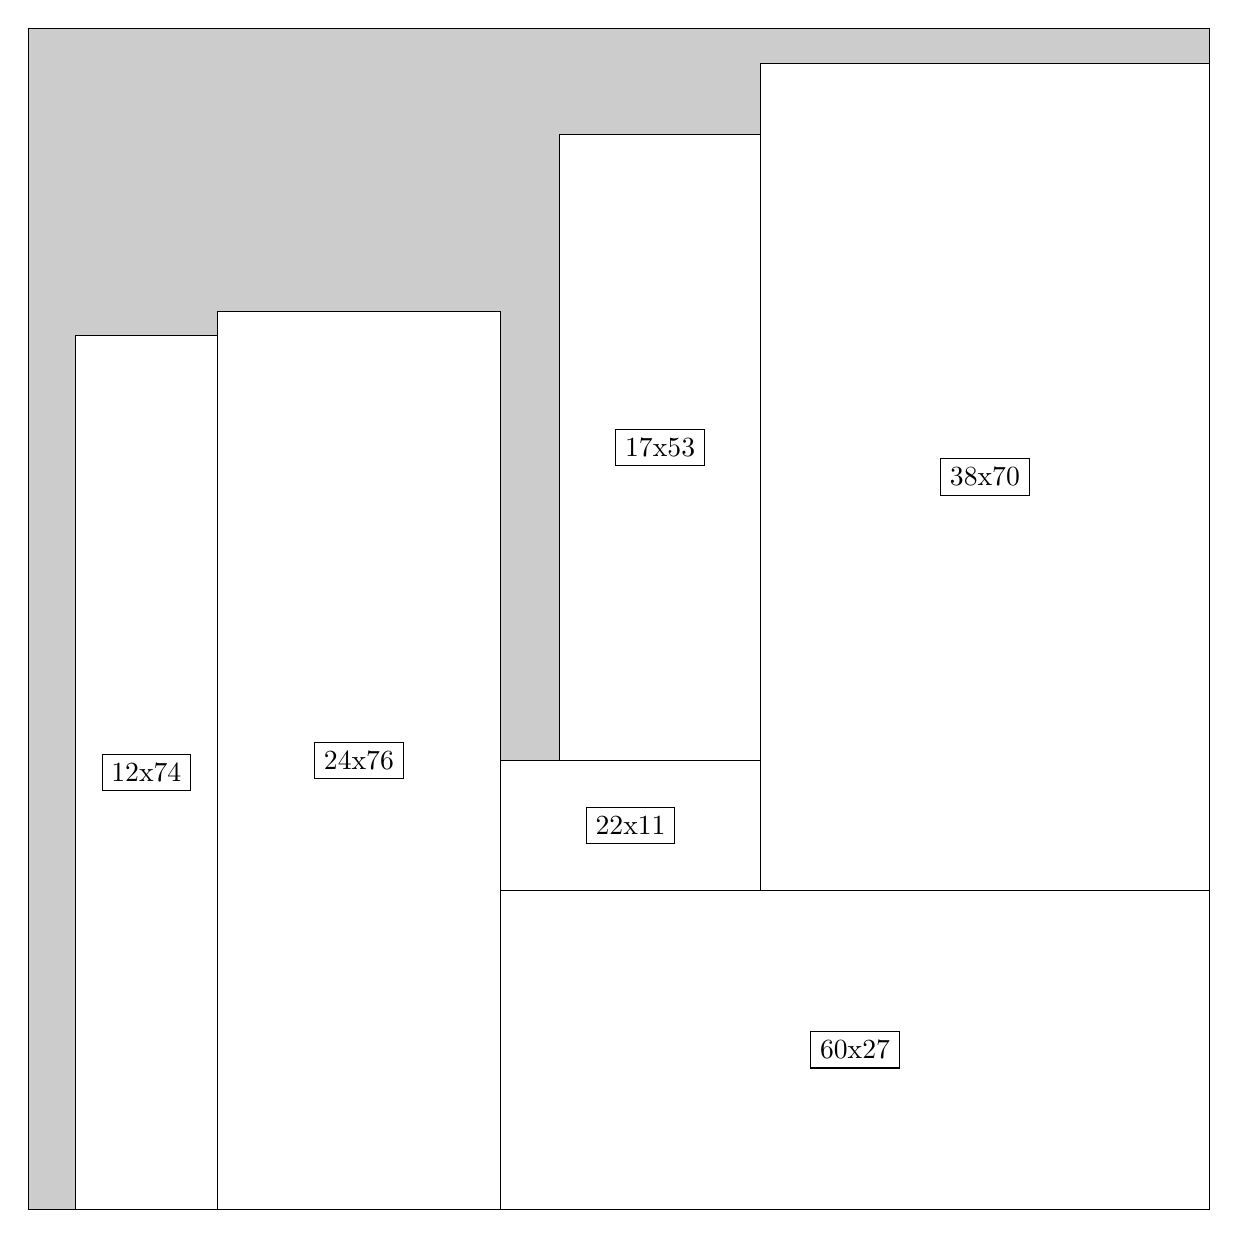
\begin{tikzpicture}[shorten >=1pt,scale=1.0,every node/.style={scale=1.0},->]
\tikzstyle{vertex}=[circle,fill=black!25,minimum size=14pt,inner sep=0pt]
\filldraw[fill=gray!40!white, draw=black] (0,0) rectangle (15.0,15.0);
\foreach \name/\x/\y/\w/\h in {60x27/6.0/0.0/9.0/4.05,38x70/9.299999999999999/4.05/5.7/10.5,22x11/6.0/4.05/3.3/1.65,17x53/6.75/5.7/2.55/7.949999999999999,24x76/2.4/0.0/3.5999999999999996/11.4,12x74/0.6/0.0/1.7999999999999998/11.1}
\filldraw[fill=white!40!white, draw=black] (\x,\y) rectangle node[draw] (\name) {\name} ++(\w,\h);
\end{tikzpicture}


w =60 , h =27 , x =40 , y =0 , v =1620
\par
w =38 , h =70 , x =62 , y =27 , v =2660
\par
w =22 , h =11 , x =40 , y =27 , v =242
\par
w =17 , h =53 , x =45 , y =38 , v =901
\par
w =24 , h =76 , x =16 , y =0 , v =1824
\par
w =12 , h =74 , x =4 , y =0 , v =888
\par
\newpage


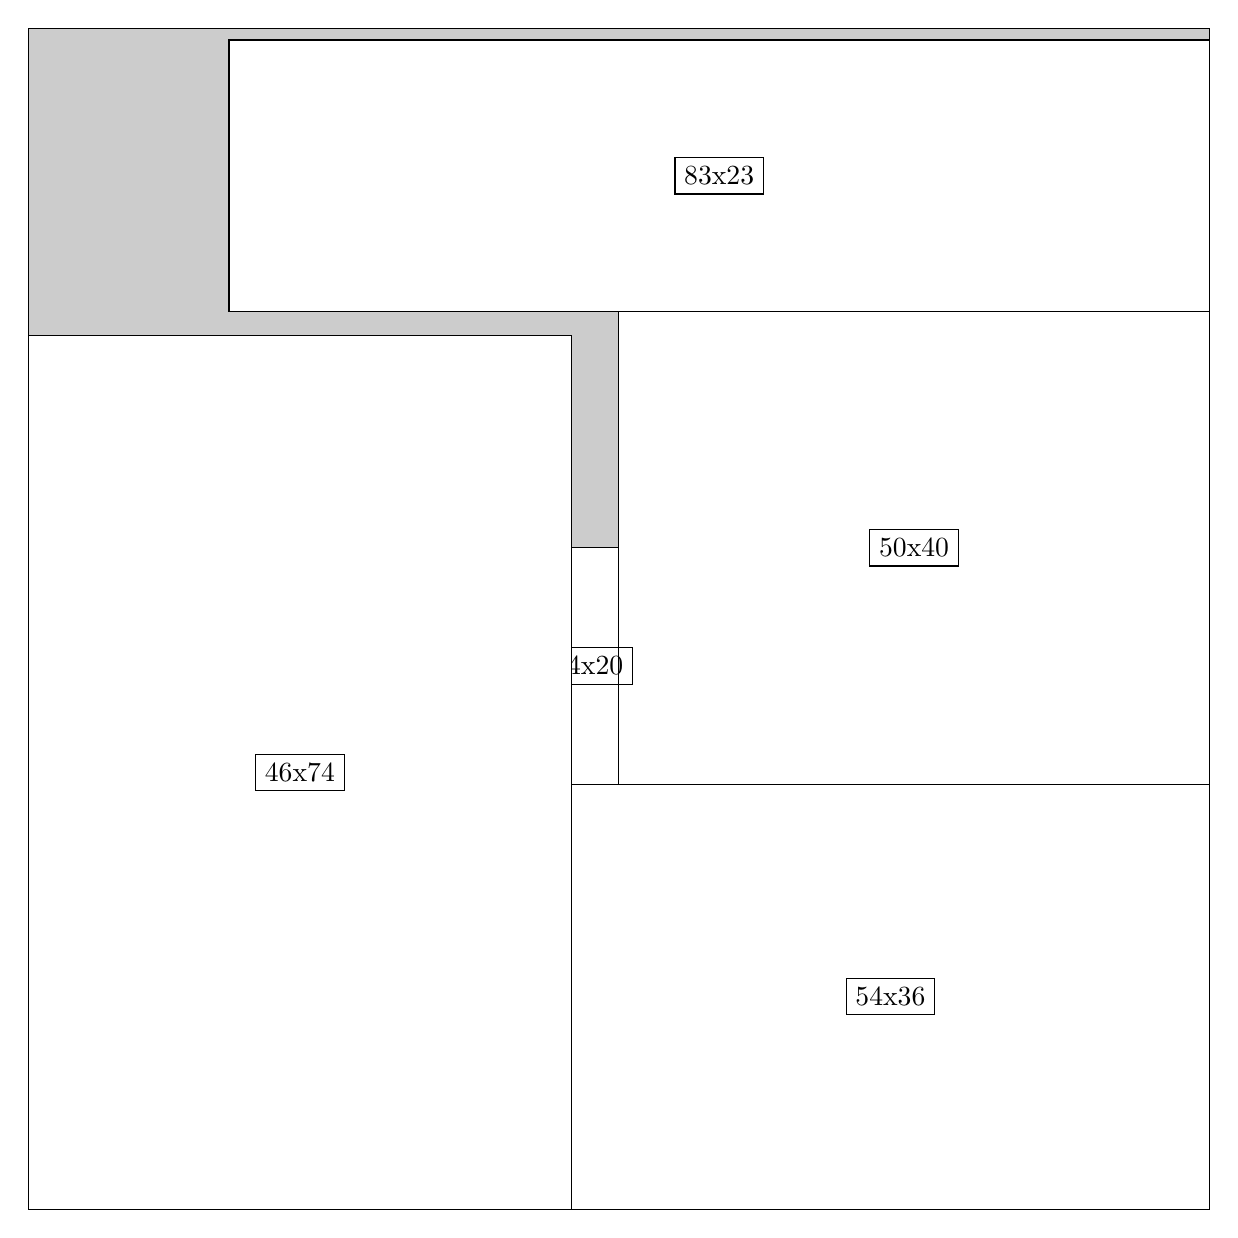
\begin{tikzpicture}[shorten >=1pt,scale=1.0,every node/.style={scale=1.0},->]
\tikzstyle{vertex}=[circle,fill=black!25,minimum size=14pt,inner sep=0pt]
\filldraw[fill=gray!40!white, draw=black] (0,0) rectangle (15.0,15.0);
\foreach \name/\x/\y/\w/\h in {54x36/6.8999999999999995/0.0/8.1/5.3999999999999995,50x40/7.5/5.3999999999999995/7.5/6.0,4x20/6.8999999999999995/5.3999999999999995/0.6/3.0,46x74/0.0/0.0/6.8999999999999995/11.1,83x23/2.55/11.4/12.45/3.4499999999999997}
\filldraw[fill=white!40!white, draw=black] (\x,\y) rectangle node[draw] (\name) {\name} ++(\w,\h);
\end{tikzpicture}


w =54 , h =36 , x =46 , y =0 , v =1944
\par
w =50 , h =40 , x =50 , y =36 , v =2000
\par
w =4 , h =20 , x =46 , y =36 , v =80
\par
w =46 , h =74 , x =0 , y =0 , v =3404
\par
w =83 , h =23 , x =17 , y =76 , v =1909
\par
\newpage


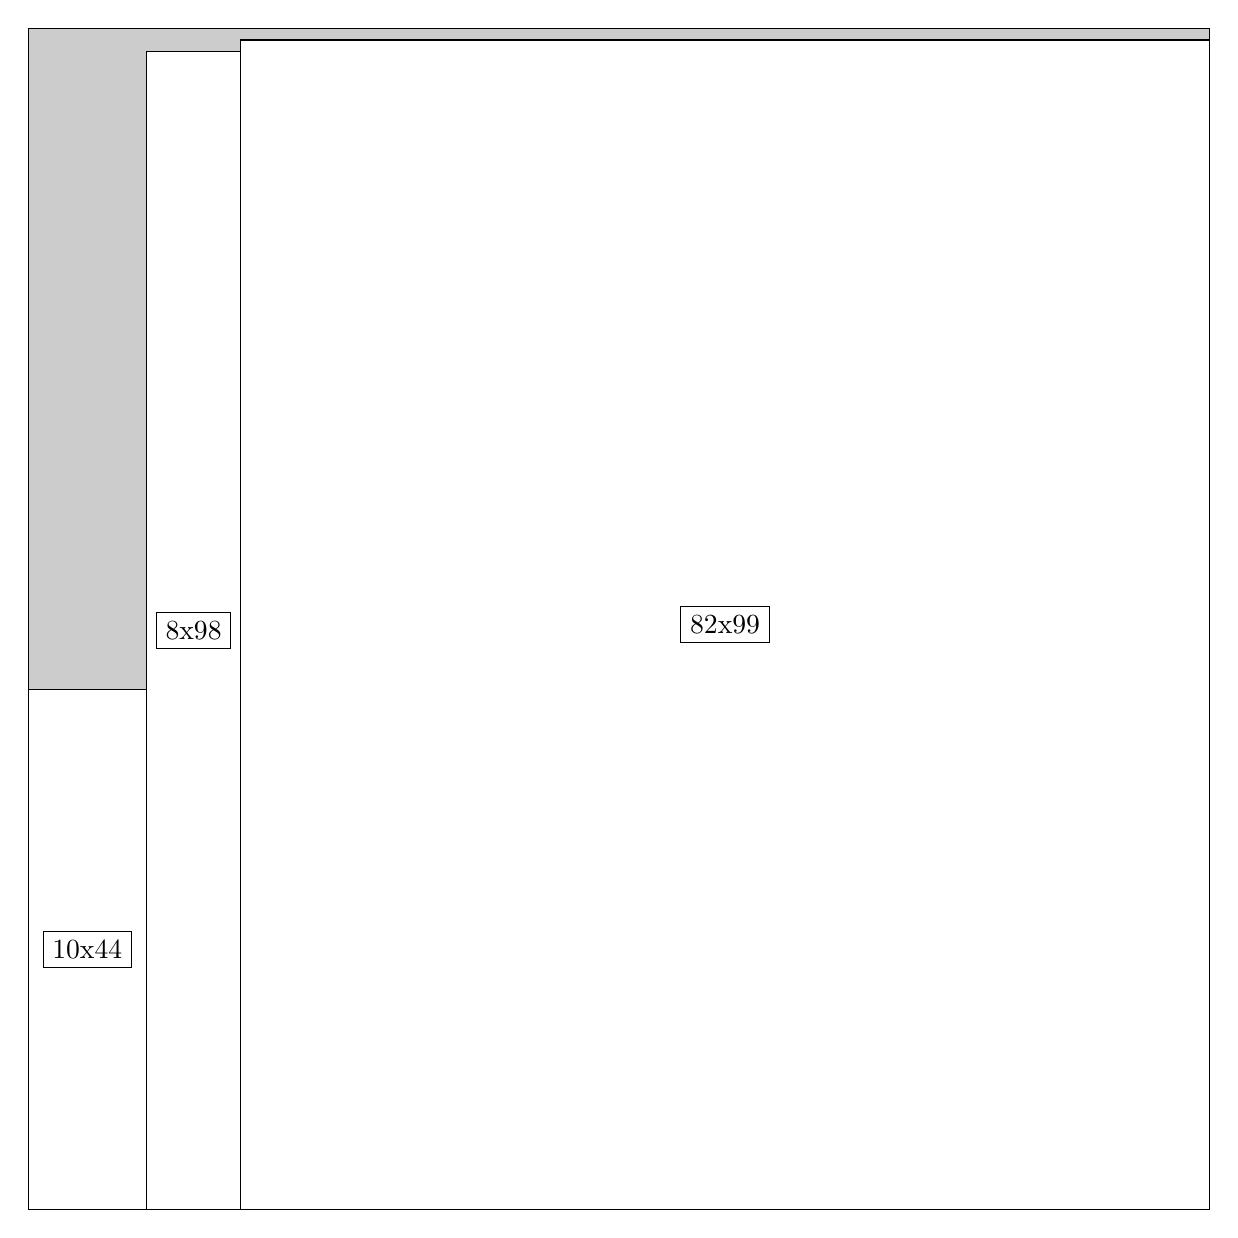
\begin{tikzpicture}[shorten >=1pt,scale=1.0,every node/.style={scale=1.0},->]
\tikzstyle{vertex}=[circle,fill=black!25,minimum size=14pt,inner sep=0pt]
\filldraw[fill=gray!40!white, draw=black] (0,0) rectangle (15.0,15.0);
\foreach \name/\x/\y/\w/\h in {82x99/2.6999999999999997/0.0/12.299999999999999/14.85,8x98/1.5/0.0/1.2/14.7,10x44/0.0/0.0/1.5/6.6}
\filldraw[fill=white!40!white, draw=black] (\x,\y) rectangle node[draw] (\name) {\name} ++(\w,\h);
\end{tikzpicture}


w =82 , h =99 , x =18 , y =0 , v =8118
\par
w =8 , h =98 , x =10 , y =0 , v =784
\par
w =10 , h =44 , x =0 , y =0 , v =440
\par
\newpage


\end{document}